O acompanhamento é pautado nos níveis de SpO$_2$ detectados pelo SMA-oxímetro; com a triagem feita de forma autonoma pelo sistema. graças à sociedade de agentes embarcada no microcontrolador. 
O SMA faz o monitoramento integral do enfermo, mantendo uma rede de apoio e um responsável técnico (médico) cientes de casos críticos. 
O fluxo de interação entre usuários e o SMA está disposto na Figura~\ref{fig:fig1}.

\begin{figure}[H]
  \centering
  \includegraphics[width=0.5\textwidth]{assets/img/interações.png}
  \caption{Diagrama de Interações}
  \label{fig:fig1}
\end{figure}

A medição é feita estabelecendo a comunicação entre os componentes do microcontrolador e o programa AgentSpeak; que é feita pela compilação do \textit{firmware} do Arduino, ARGO \cite{ArgoAgent}, na ChonIDE. A inicialização das percepções do \textit{hardware} também é feita na IDE, pelo botão de \textbf{\textit{Play}}, sendo o valor de saturação padrão 98\%, nível considerado normal em indivíduos saudáveis \cite{collins2015relating}.

Alterações nos níveis de SpO$_2$ podem ser observadas durante a interação do usuário com o teclado LCD, sendo o botão direito responsável pelo incremento e o esquerdo, pelo decremento no percentual de saturação, respectivamente.

O sistema, durante a percepção, baseando-se nos níveis de SpO$_2$ começa a efetuar o diagnóstico inicial e comunicar o quadro de risco correlato à leitura ao agente \textbf{monitor}, que exibe essa informação no console da aplicação. A classificação de risco efetuada pela aplicação é ilustrada na  Tabela~\ref{tab:tabela1}


\begin{table}[ht]
    \centering
    \begin{tabular}{|c|c|c|}
        \hline
        \textbf{Risco} & \textbf{Mínimo (\%)} & \textbf{Máximo (\%)} \\
        \hline
        Normal & 96 & 100 \\ 
        \hline
        Alerta & 90 & 95 \\ 
        \hline
        Crítico & 0 & 89 \\ 
        \hline
    \end{tabular}
    \caption{Indicadores de Risco SpO$_2$ (adaptado)\cite {kadarinaMonitoringHeartRate2018}}
    \label{tab:tabela1}
\end{table}

Casos considerados críticos são comunicados ao agente \textbf{mensageiro}, cuja responsabilidade é identificar a rede de apoio atrelada ao paciente e disparar mensagens acerca de seu quadro de saúde. Esse cenário pode ser observado nas Figuras~\ref{fig:fig2} e~\ref{fig:fig3}

\begin{figure}[H]
  \centering
  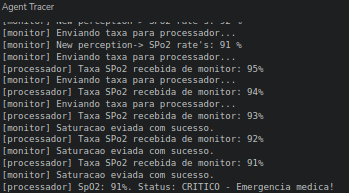
\includegraphics[width=0.99\textwidth]{assets/img/perception.emergency - Copia.png}
  \caption{Estado Crítico}
  \label{fig:fig2}
\end{figure}


\begin{figure}[H]
  \centering
  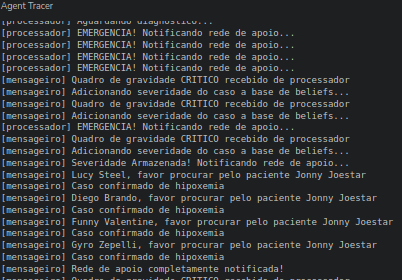
\includegraphics[width=0.99\textwidth]{assets/img/netwokcall - Copia.png}
  \caption{Contactando Rede}
  \label{fig:fig3}
\end{figure}

O modelo conceitual da arquitetura de responsabilidade única usado na construção do oxímetro está ilustrado na Figura~\ref{fig:fig4}. 
No diagrama está disposto todo o fluxo de interação e processamento de dados feito pelo oxímetro, desde a etapa de coleta até a mensageria.

\begin{figure}[H]
  \centering
  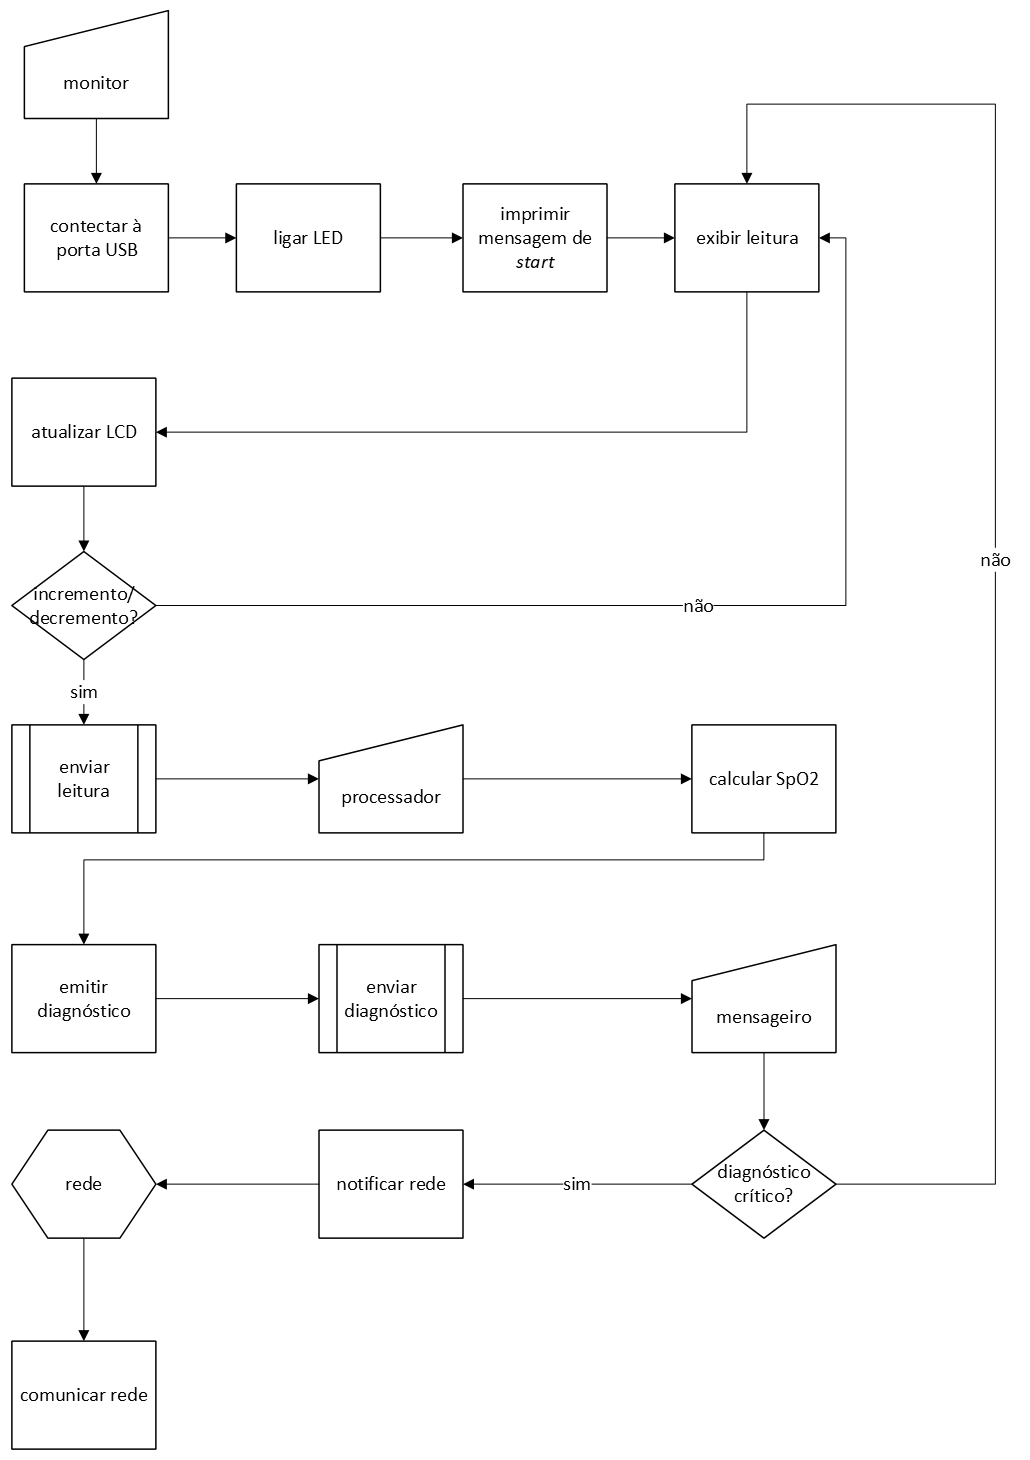
\includegraphics[width=0.9\textwidth]{assets/img/diagrama.png}
  \caption{Arquitetura Conceitual}
  \label{fig:fig4}
\end{figure}